%%%%%%%%%%%%%%%%%%%%%%%%%%%%%%%%%%%%%%%%%%%%%%%%%%%%%%%%%%%%%%%%%%%%%%%%%%%%%%%%
%2345678901234567890123456789012345678901234567890123456789012345678901234567890
%        1         2         3         4         5         6         7         8

\documentclass[letterpaper, 10 pt, conference]{ieeeconf}  % Comment this line out
                                                          % if you need a4paper
%\documentclass[a4paper, 10pt, conference]{ieeeconf}      % Use this line for a4
                                                          % paper

\IEEEoverridecommandlockouts   
\usepackage{booktabs}
% This command is only
                                                          % needed if you want to
                                                          % use the \thanks command
\overrideIEEEmargins
% See the \addtolength command later in the file to balance the column lengths
% on the last page of the document



% The following packages can be found on http:\\www.ctan.org
\usepackage{graphicx} % for pdf, bitmapped graphics files
%\usepackage{epsfig} % for postscript graphics files
%\usepackage{mathptmx} % assumes new font selection scheme installed
%\usepackage{times} % assumes new font selection scheme installed
%\usepackage{amsmath} % assumes amsmath package installed
%\usepackage{amssymb}  % assumes amsmath package installed
\usepackage{cite} % takes care of citations

\title{\LARGE \bf
"The smell of fear" - In Search of Patterns Between Emotions and Breath Composition - Literature Survey
}


\author{Jason Tam$^{1}$\thanks{{\tt\small $^{1}$jtam013@aucklanduni.ac.nz}}, Musa Abdel-Rahman$^{2}$\thanks{{\tt\small $^{2}$mabd292@aucklanduni.ac.nz}}, Catherine Liu$^{3}$\thanks{{\tt\small $^{3}$cliu129@aucklanduni.ac.nz}}\\Supervised by J{\"o}rg Wicker}

\begin{document}

\maketitle
\thispagestyle{empty}
\pagestyle{empty}

%%%%%%%%%%%%%%%%%%%%%%%%%%%%%%%%%%%%%%%%%%%%%%%%%%%%%%%%%%%%%%%%%%%%%%%%%%%%%%%%

%\begin{abstract}

%This is where the abstract goes, if we decide to have one

%\end{abstract}

%%%%%%%%%%%%%%%%%%%%%%%%%%%%%%%%%%%%%%%%%%%%%%%%%%%%%%%%%%%%%%%%%%%%%%%%%%%%%%%%

\section{INTRODUCTION}

An important process of many biological organisms is gas excretion. The gas excretions of humans compose of Carbon Dioxide and various Volatile Organic Compounds (VOCs) such as isoprene and acetone. These VOCs have been found to play an important role in the communication between plants, and even between plants and animals, however we do not know if these VOCs have any impact on human communication. Research within the field to understand how these VOCs interact or are correlated with human emotions have been attempted by \cite{NATURE}.

The intention of this study is to continue on from the accomplishments mentioned in \cite{NATURE}. The current plan is to further explore the potential patterns/associations that are intrinsically present in the collected dataset, starting with general pattern mining strategies with unsupervised learning techniques, and may apply supervised learning methods for finer details of the resulting patterns if feasible. This paper explores techniques that are potentially useful for various analysis possibilities of the data, such as using \textit{Dynamic time warping} to align different sessions of the same movie, or clustering techniques that may reveal high volume detection in certain molecular mass channels are trigged by certain scene types.

%An idea could be to examine the time trends of different gases of the same movie, to attempt in identifying relationships between molecular masses and certain emotions/theme of movie. 

%Also time segments from all movies with the same scene category can be grouped together to examine the statistics of different molecular masses, possibly with time lags between the movie scene and the detection time. Clustering techniques can be useful 

%Dynamic time warping can potentially be used to align different sessions of the same movie for analysis.

%Also got another idea from Joerg. First tally up the frequency of different scene categories in each of the movies (such as 3 action scenes and 2 romantic scenes), then perform data mining against the total (relative) tally of the detected gas in each of the channels.

%%%%%%%%%%%%%%%%%%%%%%%%%%%%%%%%%%%%%%%%%%%%%%%%%%%%%%%%%%%%%%%%%%%%%%%%%%%%%%%%

\section{PREVIOUS WORK ON THE SUBJECT}
\subsection{Breath Composition and Emotional States}
Previous research has already been conducted in this area to try and identify and understand VOCs and the impact they have on a person's emotional state \cite{NATURE} \cite{Wicker:2015:CDM:2783258.2783404}. Within these studies, Wicker et al utilized data collected from a cinema in Mainz, Germany which included concentrations of VOCs in the cinema, and also information on the content of the movie at the time of each measurement (this was given the variable 'scene label').  From this, they tried to identify the relationship between VOC concentrations and the 'scene labels'. Four approaches were used to analyze the data sets:
\begin{itemize}
	\item Using regression to predict future VOC concentrations given the past VOC concentrations and scene labels (forward prediction)
	\item Using abductive reasoning to help predict past scene labels from future VOC concentrates (backward prediction)
    \item Validation of predictions using forward learners as input to the backward learners
    \item Using a modified Granger causality methodology where comparisons are made between performance with and without a particular time series
\end{itemize}

Ten minute time frames were examined as various factors were taken into consideration such as the delay in time for the breath gases to reach the mass spectrometer, external factors such as audience influences, or the misalignment of data. Within the first method of forward prediction, trees were utilized to help explore and understand the data, as this helped to show dependencies that occurred within the data especially in understanding what scenes made particular VOC concentrations go up. Abductive reasoning was used in the second approach to explore relationships and to validate the prediction of future events in time series. Again, trees were utilized to help visualize any dependencies or any relationships. Random Forest algorithms were used to construct models for each mass, CO$_2$ and scene labels. Using these methods it was found that good models could be trained on those variables that evoked strong emotional responses, such as blood, and death scenes.  This was proven to be the case both in repeat screenings of the same movie or within different films with the same scene label. 

It may be beneficial for us to utilize regression models and trees to find relationships within our data sets as this is a simple and easy way to understand any relationships that may occur, which can also be easily explainable. However, it is important to remember that when using random forests to construct our models, that thorough data preparation has been undertaken as random forests have been observed to over-fit for some datasets with noisy classification or regression tasks.  

\subsection{Gas Sensing Systems and Emotion Recognition}
Takahashi and Sugimoto \cite{4601732} also conducted similar experiments in which they used a smart gas sensing system to achieve emotion recognition using breath composition.  The gas sensing system was comprised of a sensor that was made using a quartz crystal resonator with plasma-polymer film. This sensor was able to pick up VOCs under dry air conditions. They collected samples from 20 subjects, who partook in questionnaires that were based on the multiple mood scale. The questions evoked emotions, which in turn were captured using the smart gas sensing system. A dental rinse was used to excite the emotion, and readings were taken before and after using this rinse.  From this, two emotions, comfortableness (having a positive emotion and feeling refreshed) and no emotion were considered. Using this data, machine learning approaches were utilized to explore and validate if breath composition was feasible for emotion recognition.

Takahashi and Sugimoto first explored using Neural Networks to explain their data.  A (16-12-8-6-2) network was used, where the activation function of the neurons was a linear function in both the input and output layers, and a sigmoid function applied to the hidden layers. Trial and error was used to find the number of neurons they would use in the hidden layers. A 'leave-one-out' cross-validation was employed to evaluate the validity of the model. From this the average recognition rate was 47.5\%, with the detection of comfortableness being 55\%, and having no emotion resulted in an even lower recognition rate and was a lot harder for the Neural Network to detect. Support Vector Machines (SVM) were also utilized to test emotion recognition from breath gas information. During the emotion recognition process, the feature vector was fed into the SVM and the output from the SVM investigated in the decision logic that selected the best emotion, and the class of the SVM indicated the recognition result.  The kernel function used a gaussian function and the margin parameter and function parameter were defined by trial and error.  Again, the 'leave-one-out' cross-validation method was used to evaluate the validity of the model. From this, a higher average recognition rate of 67.5\% was achieved.  

Following this, Takahashi and Sugimoto extended the aforementioned research by introducing another emotion into the experiment - displeasure \cite{Takahashi2008}.  In terms of experiment methodology, all equipment and testing were kept constant to the previous study. Again, Neural Networks were employed in trying to achieve emotion recognition using breath gas information. In alignment with Takahashi and Sugimoto's previous study, it was found no emotion was hard to recognize, and after the introduction of displeasure into this experiment, this too was also hard for the neural network to recognize. In the neural networks explored, the output layer contained 3 neurons with varying results for average emotion recognition based on the neural network structure.  It was found a (7-11-11-3) network had less than 50\% success rate for the average recognition rate.  This average recognition rate increases to 75\% once a (14-14-6-3) network is introduced, however this comes at the expense of a reduced rate of pleasure recognition.  Again, the number of neurons in the hidden layers and the learning factors were deemed through trial and error in order to converge the learning of the neural network. 

Within the SVM model, the 'one-vs-all' method was utilized due to the multiclass classification of the dataset. Moreover, the feature vector was fed into the SVMs during the emotion recognition process, and the output from each SVM was investigated in the decision logic that selects the best emotion.  A 3rd order polynomial was used as the kernel (and c as 1 and 10 for the two models they fit) and trial and errors used to find other parameters in order to give the training data a complete classification rate. The best performing SVM model that Takahasi and Sugimoto created had an average recognition rate of 83\% -higher than the neural network model and also higher than the previous SVM models they made when only two emotional states were explored. 

Through both these experiments \cite{4601732} \cite{Takahashi2008}, the results suggest that machine learning models could be employed to understand and predict emotion through breath gas information. In both the Neural Network and SVM models, we see a lot of trial and error is involved in computing the parameters involved to obtain the best average recognition rates. This can be a tedious process and would need to be recalculated whenever new data was uploaded and require much more expertise to tune. Within the Neural Network, we see advantages as the architectures can be easily adapted to any situation and their hidden layers reduce the need for feature engineering. However, they are computationally intensive to train, and they require much more expertise to tune. SVM models are also hard to tune due to the importance of picking the right kernel and may not scale well to larger or other data sets, so this will need to be taken into consideration. Once all these factors are taken into consideration, these supervised learning techniques may still be beneficial for us to utilize with our data set if we already know what we wish to classify or predict.

\subsection{Classification of Emotional Biosignals}
Similar work was done by Frantzidis et al \cite{5373931} where data mining was utilized to explore the classification of emotional biosignals that were evoked through pictures selected from the International Affective Picture System (IAPS).  The IAPS pictures were rated in terms of valence (pleasure) and arousal. Using data mining techniques in the way of a C4.5 decision tree algorithm, the biosignals were classified according to their valence dimensions.  These, along with the gender of the subject, became inputs that were fed into a Mahalanobis classifier which categorized the data into high and low arousal. Using this combined data mining and pattern recognition technique saw an average recognition rate of 77.68\% for the four emotional states (these states differed both in their arousal and valence dimensions). 

This experiment looks at supervised learning once classifications for the data set have been made, and uses combined methodologies to arrive at the average recognition rates.  This is helpful to note and utilize in further work as most data preparation, transformation and modeling may go through many iterations and many different models before coming to a result we are happy with. Using a C4.5 decision tree is any easy way to come to an easily interpretable classification however it is important to know and understand the data you are working with, as small variations in the data can lead to different decision trees.  This would mean that very different results could be concluded each time a different data set was run. It can be seen in both this project and the aforementioned project by Wicker et al \cite{NATURE} \cite{Wicker:2015:CDM:2783258.2783404} that employing trees in interpreting and understanding relationships between the data could be a great first step in explanatory analysis for our project.
 
\subsection{Data Analysis on VOCs}
It was found that Electric nose systems, (an instrument consisting of an array of reversible but only semi-selective gas sensors coupled to a pattern recognition algorithm) (also known as e-noses) have been widely used for the analysis of VOCs \cite{Scott2006}.  Scott, James and Ali offer various ways in which the data analysis from these systems can be analyzed, which will be explored further in this literature review. It is essential to combine many analytical techniques together to help classify data as more often than none relevant data may be lost when trying to reduce the dataset on a whole. It is interesting to note that the classification algorithm chosen to model the data is very important - choosing a poor algorithm results in a model that may lack the ability to model non linear data, or it may result in an over trained and over-fit model.  

%%%%%%%%%%%%%%%%%%%%%%%%%%%%%%%%%%%%%%%%%%%%%%%%%%%%%%%%%%%%%%%%%%%%%%%%%%%%%%%%

\section{MACHINE LEARNING}

Machine learning \cite{geron2017hands} is a field of data science that focuses on 'machines' extracting relationships/patterns that are intrinsically present in data. 'Machines' refers to all systems that can make use of algorithms to perform computations, as well as the ability to store and recall the intermediate results of such computations in order for final solutions to converge. It is an extension on the traditional methods from statistics with concepts from artificial intelligence, and the techniques used to process data can generally be categorized into \textit{supervised} and \textit{unsupervised} learning. Supervised learning represents scenarios where a target response variable is present within the data, and chosen algorithms are to determine how the target response is affected by the other input variables in the data. The result would provide a logic that determines a likely output when a new input value is given, which could be labels with classification algorithms or numerical values with regression algorithms. Unsupervised learning represents scenarios where a target response is not specified, and the algorithm is to determine if any underlying patterns/relationships are present in the data, which is treated as unstructured noise. 

The objective of this study is centred around determining potential relationships between breath composition and emotion, via a collected dataset that contains gas composition detected in cinema sessions of different movie types. While there is no clear target response variable for the analysis to predict, one can assume it might be possible to predict the traces of some molecular masses that would be captured by the VOC device once enough patterns are extracted the data, given the attendance data and scene categorizations of the movie.

\subsection{Supervised Learning}

Techniques that are categorized as supervised learning \cite{geron2017hands} are useful when the target response variable is included in the input to the algorithm. This approach aims to determine the relationship between the target response and the other variables in the data, and use it for prediction on new input variables. Common techniques include ones that are traditionally from the statistics domain, such as \textit{linear regression} and \textit{logistic regression}, as well as ones that are later developed under the data science domain such as \textit{k-nearest neighbour}, \textit{random forests}, \textit{decision trees}, \textit{support vector machines} and \textit{neural networks}.

This approach is most commonly used in analysis where obtaining accurate predictions have the highest priority, while the explanation of the results is often secondary. For this reason, such analysis often take the approach of partitioning the data into training and testing sets. Building independent prediction models using different methods with the training data, and choose the one with the best prediction performance using the testing data. As most of the algorithms that were developed outside of the traditional statistics domain favours prediction in the expense of explanation (which are often referred to as 'black box methods'), hence such techniques are often avoided when causal inference is required as part of the analysis result.

\subsection{Unsupervised Learning}

Unsupervised learning \cite{Gentleman2008} covers a broad range of algorithm concepts, with each of them emphasized in certain strengths. Almost all of them share a common philosophy, which is essentially determining a probabilistic model for new input variables based on the existing data. For simpler cases where the data is \textit{unstructured}, which means the order of the input's arrival is irrelevant, one can assume that they are all drawn independently from the same underlying distribution $P(x)$ in an identical manner. This setting is particularly useful for analysis objectives such as \textit{outlier detection} or general \textit{monitoring}. \textit{Classification} problems can also make use of this by determining a probability distribution for each of the labels in existing data, which are then used to classify the new inputs based on their attributes. While such a framework can be applied to a wide range of models, the objective in the practice of machine learning remains to be finding/developing models that are most appropriate for the data set to be analyzed while being aligned with certain predetermined goals. 

\subsection*{Latent Variable Models}

There are some techniques that are used to construct probabilistic models based on some latent or hidden variables, which are quite commonly used when performing \textit{dimensional reduction} and \textit{clustering}, considered corner stones of unsupervised learning.

\textit{Factor Analysis} is a popular method used to deal with high-dimensional datasets. Datasets that have high number of dimensions may sometimes be a real challenge for the machines, because there can be too many parameters to reliably estimate even with the simplest algorithms. Factor analysis makes use of multivariate gaussian vectors to estimate a gaussian density for high dimensional data, and provide a low-dimensional representation of the data and associated results. \textit{Independent Components Analysis (ICA)} is an extension to this technique that deals with data with factors that are not gaussian-distributed, which is suitable for many real world datasets that often have a certain degree of sparseness.

\textit{Principal Component Analysis (PCA)} is another common method used to simplify high-dimensional data. It transforms a set of observations that are possibly correlated into a set of linearly independent ones, which are termed \textbf{principal components}. This resulting set is often used as input to other algorithms, and their linear independence often assist greatly in reducing calculation complexity.

Mixtures of such gaussian distribution are made use in clustering algorithms such as \textit{K-means}. Datasets containing $n$ observations are partitioned in to $k$ clusters, where each observation would belong to the cluster with the nearest mean. This is achieved by estimating the maximum likelihood parameters using the iterative algorithms such as the \textit{Expectation-maximization} algorithm. This is commonly used in preprocessing steps to determine initial configurations for other algorithms.

\subsection*{Time Series Models}

While there are possible approaches to partition the dataset in a time-independent manner for this study, the observations are nevertheless collected sequentially, which potential underlying patterns may exist. Traditional methods in statistics such as the \textbf{A}uto\textbf{R}egessive \textbf{I}ntegrated \textbf{M}oving \textbf{A}verage (ARIMA) methods \cite{bontempi2012machine} construct probabilistic models for present and future observations with past observations. \textit{State Space Models} (SSM) and \textit{Hidden Markov Models} (HMM) are also common methods used to process time-series data, where they assume the observed is a consequence of data in hidden states. 

%%%%%%%%%%%%%%%%%%%%%%%%%%%%%%%%%%%%%%%%%%%%%%%%%%%%%%%%%%%%%%%%%%%%%%%%%%%%%%%%

\section{DYNAMIC TIME WARPING}

\textit{Dynamic Time Warping} \cite{berndt1994using} is a technique developed to analyze time series data, with initial inspirations from concepts in studies of speech recognition. Word recognition is mostly performed by matching existing templates in a library to the time series speech data recorded. The time axis of either sequence is often adjusted by either elongation or compression to minimize some distance measure for the two data sets to be as aligned as possible.

\begin{figure}[thpb]
  \centering
  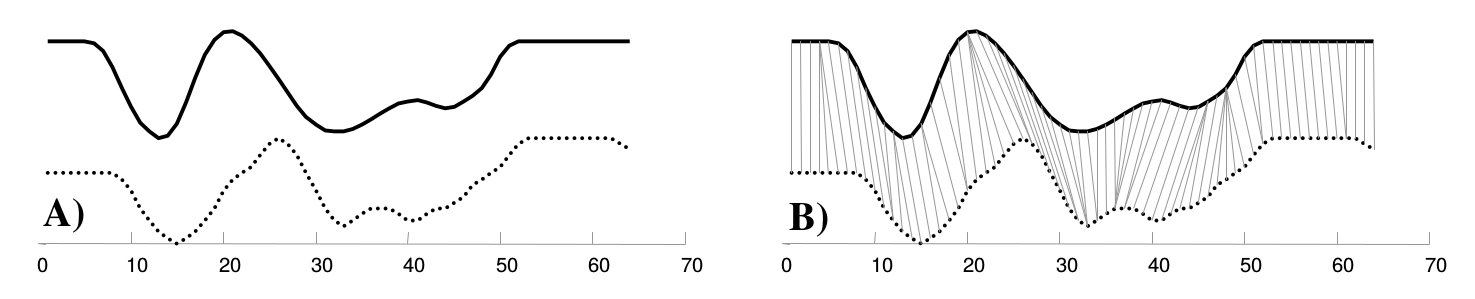
\includegraphics[width=0.47\textwidth]{DTWOne.png}
  \caption{A visualization of the main mechanism in the Dynamic Time Warping technique. \cite{doi:10.1137/1.9781611972719.1}}
  \label{DTWOne}
\end{figure}

Figure \ref{DTWOne} shows an example from \cite{doi:10.1137/1.9781611972719.1} of the utility of dynamic time warping. Figure \ref{DTWOne} A) presents the vertical position of an individual's hand while expressing the word "pen" in Sign language in two separate scenarios. While an observable level of similarity is present between the two sequences, a simple approach of assuming the i$^{th}$ point on one sequence is aligned with i$^{th}$ point on the other will produce a pessimistic dissimilarity. Figure \ref{DTWOne} B) presents an alignment produced by a more sophisticated distance measure.

While DTW has shown to be successful in many disciplines, it should be noted that the algorithm can sometime produce undesired results. Based on the principle that the algorithm attempts to explain variability on one axis ($Y$) by warping the other ($X$), it can often lead to unintuitive alignments where single points on one sequence would map to multiple points or a large section on the other sequence. Such points are commonly termed "singularities", and while compensative approaches have been proposed as alternatives, they in general restrict the possibilities of allowed warping configurations. It is possible that the "correct" warping might be prevented from discovery with such restrictions. Common definition for the "correct" warping is usually defined by the features being matched, such as peaks, troughs and plateaus on the sequence. This approach is efficient in producing a good alignment if the sequences are similar except for some local accelerations and decelerations in the horizontal (time) axis. Slight differences in these features between the two sequences (such as a peak being higher) may cause the algorithm to fail. This is demonstrated in Figure \ref{DTWTwo}

\begin{figure}[thpb]
  \centering
  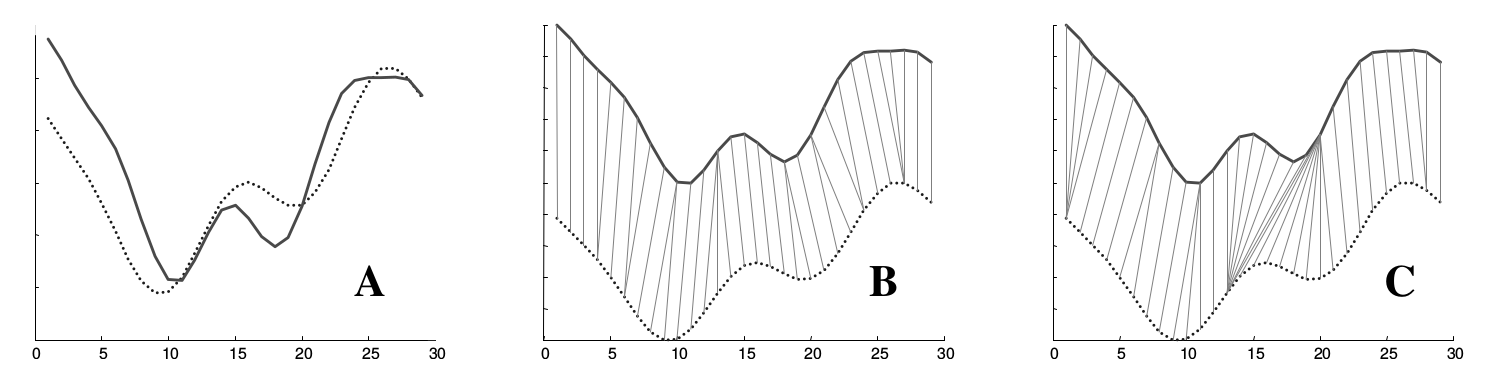
\includegraphics[width=0.47\textwidth]{DTWTwo.png}
  \caption{A visualization of the DTW mechanism failing due to difference in features between the two sequences. \cite{doi:10.1137/1.9781611972719.1}}
  \label{DTWTwo}
\end{figure}

\subsection*{Derivative Dynamic Time Warping}

While this traditional approach determines the warping factor essentially by minimizing the (typically Euclidean) distances between the two sequences, it is particularly sensitive to differences in the vertical ($Y$) axis. While differences at the global scale such as difference means, scalings or linear trends can be removed efficiently, its biggest weakness remains to be considering only the $Y$ values during the optimization process. This can often cause points on a rising trend to be mapped to a declining trend, which we would not intuitively agree. \textit{Derivative Dynamic Time Warping} is an alternative technique developed by Keogh and Pazzani \cite{doi:10.1137/1.9781611972719.1} that considers the first derivative of the sequences instead of the actual $Y$ values. They have shown in their paper that this technique is effective against scenarios describe in Figures \ref{DTWOne} and \ref{DTWTwo}. Such techniques can potentially be very useful in comparison of time segments from datasets of different movie sessions, and determining if a correlation is present between such trends.

%%%%%%%%%%%%%%%%%%%%%%%%%%%%%%%%%%%%%%%%%%%%%%%%%%%%%%%%%%%%%%%%%%%%%%%%%%%%%%%%

\section{CLUSTERING AND PATTERN CLASSIFICATION}

Clustering data into groups based on similarity is often one of the most important steps in any data-analysis application. Currently, most clustering algorithms partition the data into groups that are disjoint, while other algorithms extend this approach to probabilistic or overlapping clustering \cite{Ramasubramanian2017}. The goal of data clustering is to identify homogeneous groups or clusters from a set of objects. In other words, data clustering aims to divide a set of objects into groups or clusters such that objects in the same cluster are more similar to each other than to objects from other clusters \cite{Hastie2009}. Some researchers present cluster analysis as part of broader features analysis of data and break it into clusters, it may include some of them of or all \cite{Ramasubramanian2017}:
\begin{itemize}
	\item  Factor analysis: Where we first reduce the dimensionality of data
	\item Clustering: Where we create clusters within data
    \item Discriminant analysis: Measure how well the data properties are captured
\end{itemize}  
Many important applications, like e-nose systems, generate data that has a set of dependent variables and semi-independent variables, and the data vectors \cite{Scott2006}. The goal is to uncover disparate and hidden relations between them, by using different types of exploratory and confirmatory techniques to recognize patterns. It is also useful when we have data vectors with no descriptors, therefore similarities between classes to define groups, classes, and patterns will be used, as there would not be any feedback about classes before \cite{Hastie2009}. Similarity is usually measured by a distance function defined on pairs of patterns. As there are a wide variety of feature types and scales, the distance measure should be chosen carefully. It is most common to calculate the dissimilarity between two patterns using a distance measure defined on the feature space  \cite{Scott2006}. A good clustering algorithm can be evaluated based on two primary objectives \cite{Ramasubramanian2017}:
\begin{itemize}
	\item High intra-class similarity
	\item Low inter-class similarity 
\end{itemize}

	 Many Pattern recognition Techniques  have been developed in the past, and typically classified as below, based on what we assume for our underlying data \cite{Ramasubramanian2017}
 \begin{table}[ht]
  \caption{Pattern recognition}
  \label{Pattern recognition Techniques}
  \begin{center}
    \begin{tabular}{|c|c|c|}
      \hline
      \textbf{Technique}&\textbf{Definition}& \textbf{Example}\\
      \hline
      Connectivity Model & {\begin{tabular}[c]{@{}c@{}}Distance Connectivity \\ between Observations\end{tabular}}  &  \multicolumn{1}{c|}{\begin{tabular}[c]{@{}c@{}}Hierarchical\\ Cluster Analysis\end{tabular}}\\
\hline Centroid Models&{\begin{tabular}[c]{@{}c@{}} Distance from mean value\\ observation of each\\observation is the measure\end{tabular}} &\multicolumn{1}{c|}{\begin{tabular}[c]{@{}c@{}} K-means\end{tabular}}\\      
\hline classification&{\begin{tabular}[c]{@{}c@{}}  classify using  \\ majority vote\end{tabular}} &{\begin{tabular}[c]{@{}c@{}} K-nearest\\ neighbour\end{tabular}}   
\\ \hline {\begin{tabular}[c]{@{}c@{}}  linear data \\ compression\end{tabular}}& {\begin{tabular}[c]{@{}c@{}}  Significance of \\statistical distribution of \\ variables in the dataset \\is the measure\end{tabular}} &  \multicolumn{1}{c|}{\begin{tabular}[c]{@{}c@{}}Principal \\component analysis\end{tabular}}
\\ \hline
\end{tabular}
\end{center}
\end{table}
\subsection{Hierarchical Cluster Analysis (HCA)}
HCA techniques attempt to separate data into specific groups, based on a similarity measure. Initially each data point represents its own cluster, then the threshold for the decision when to declare two or more objects to be members of the same cluster is lowered incrementally \cite{Scott2006} \cite{Ramasubramanian2017}. This strategy will produce hierarchical representations in which
the clusters at each level of the hierarchy are created by merging clusters at the next lower level. At the lowest level, each cluster contains a single observation. At the highest level there is only one cluster containing all of the data \cite{Hastie2009}, and that can be graphically displayed in a \textit{Dendrogram Diagram}. This diagram will represent a Binary tree that reflect the \textit{agglomerative} and the \textit{divisive} approaches, which are used to show the similarity and dissimilarity between groups \cite{Scott2006} \cite{Hastie2009}. A visual illustration of this method is presented in Figure \ref{1234}.
\begin{figure}[thpb]
   	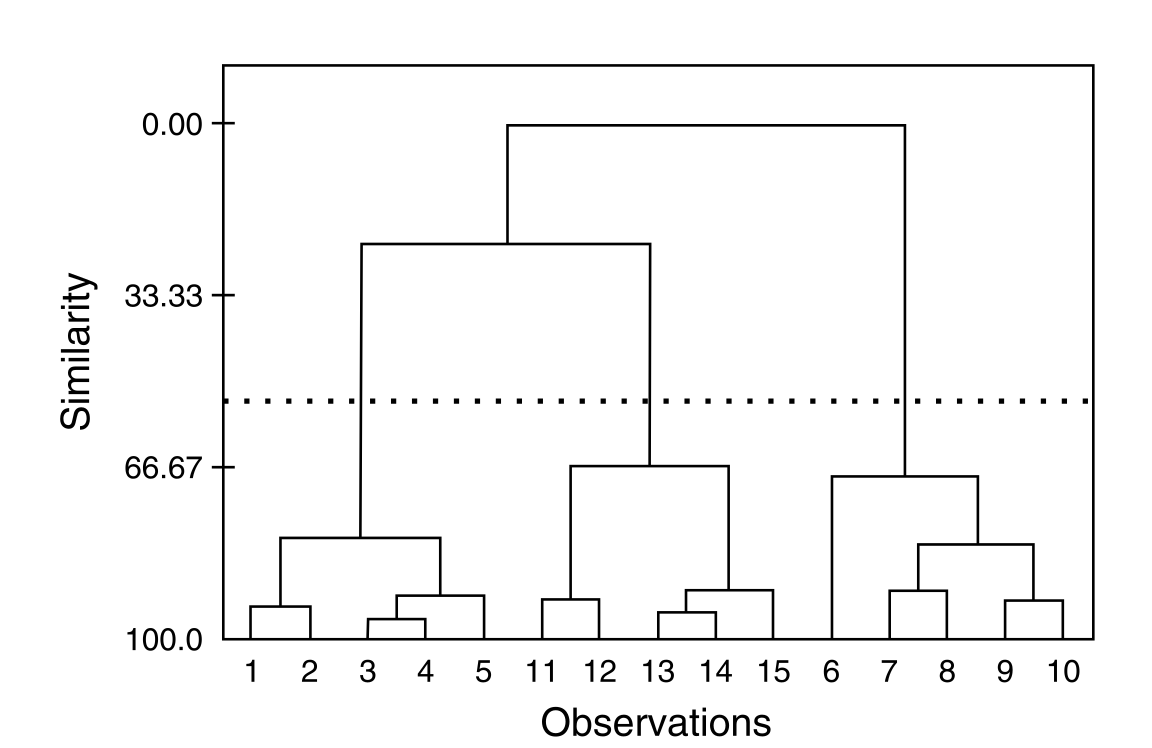
\includegraphics[width=8cm,height=3cm]{1234.png}
      \caption{Dendogram illustrating HCA data clustering\cite{Scott2006}}
      \label{1234}
   \end{figure} 
\subsection{K-means}
K-means is considered as a \textit{partitional
clustering} algorithm, which attempts to obtain partitions in the data instead of a clustering structure, but the common problem with this approach is the need to specify the desired number of clusters before computation begins. The partitional techniques usually produce clusters by minimizing a criterion function defined either locally or globally. Cluster prototypes are not usually known beforehand,
and are calculated by the algorithm simultaneously with the partitioning of the data \cite{Scott2006}. The aim of the K-means algorithm is to divide M points in N
dimensions into K clusters so that the within-cluster sum of squares is minimized. It is not practical to require that the solution has minimal sum of squares against all partitions,
except when M, N are small and K = 2. We seek instead for a "local" optima, a solution such that no movement of a point from one cluster to another will reduce the within-cluster sum of squares \cite{Ramasubramanian2017}. The K-means algorithm alternates the two steps \cite{Hastie2009}:
\begin{itemize}
\item  for each center we identify the  subset of training points (its cluster)
that is closer to it than any other center
\item the means of each feature for the data points in each cluster are
computed, and this mean vector becomes the new center for that cluster
\end{itemize}
Several variants of the k-means algorithm have been reported and many attempt to estimate a good initial partition so that the algorithm is more likely to converge at the global minimum value. Another variation of the algorithm is to split and merge the resulting clusters. This type of variant allows an optimal partition starting from almost any arbitrary initial partition, providing well-determined threshold values are
specified \cite{Scott2006}.
\subsection{K – nearest neighbour (KNN)}
KNN is an algorithm that combines regression and  classification, and is sometimes called memory-based learning, as they learn from set of events captured in the data \cite{Ramasubramanian2017}. Training the
model simply consists of storing the training data by using \textit{Euclidean} to compute similarities. The distance between an unclassified pattern vector and every sample from the training set is calculated, and it is assigned to the class of the k neighbours with the closest distances after taking the top N products based on the rating vector  \cite{Scott2006}\cite{Ramasubramanian2017}. Choosing K (classes) relies on the way that we use the algorithm. The most popular prototype is 1-NN  \cite{Scott2006}, since it gives binary classes and the boundary near to be linear \cite{Hastie2009}, but the variance is so high, so by training you can reach to optimal K. \subsection{Principal component analysis (PCA)} PCA is an unsupervised multivariate procedure and is a well known linear data compression and feature extraction technique, mainly used as a filter method to remove features without knowing the effect on the classification algorithm \cite{Hastie2009}. The scores produced may be plotted in two or three dimensions to inspect the data. PCA derives new, uncorrelated variables that are linear combinations of the original variable set ordered by reducing variability. It is mainly used to reduce the dimensionality of a data set while retaining as much information as possible by eliminating the lowest ranking variables. PCA is a simple and fast method but remains a linear approach, therefore any non-linear correlation between variables will not be retained \cite{Scott2006}.
\subsection{Applications}
According to Scott, James and Ali \cite{Scott2006}, these techniques were helpful when they implemented their data analyzing research on \textit{E-nose system}, since every one of them has a feature that supports them on their duties:

\begin{itemize}
	\item \textit{HCA}: Full structure for all clusters that generated, with complete linkage. 
	\item  \textit{PCA}: Utilizing PCA supported them to separate between groups and illustrated the interaction between them.
    \item \textit{KNN}: Feature extraction method was used based on a curve fitting model of multiple gases with KNN as the classifier.
    \item \textit{K-means}: Used as an explanatory method and it helped to detect the different behavior for some sensors based on their circumstances.
    \end{itemize}
    
%%%%%%%%%%%%%%%%%%%%%%%%%%%%%%%%%%%%%%%%%%%%%%%%%%%%%%%%%%%%%%%%%%%%%%%%%%%%%%
   
\section{CONCLUSIONS}

Through the review of previous work done within this subject area by Wicker et al \cite{NATURE},\cite{Wicker:2015:CDM:2783258.2783404} and similar fields \cite{4601732},\cite{Takahashi2008},\cite{5373931}, we have found many helpful techniques that may be useful to implement in our research.  It was found in multiple papers \cite{Wicker:2015:CDM:2783258.2783404},\cite{NATURE},\cite{4601732},\cite{Takahashi2008} that utilizing tree algorithms would be an easy way to perform variable screening or feature selection, and this would also help us understand the data and easily find relationships between variables. Takahashi and Sugimoto \cite{4601732},\cite{Takahashi2008}, employed neural networks and support vector machines to help predict emotional states and Frantzidis et al \cite{5373931} stress the importance of combining various different methodologies to arrive at the best outcome.  These are all helpful methodologies which can be explored once we have decided what we wish to predict or find within our research.

Techniques from the machine learning \cite{geron2017hands} domain incorporates methods from the statistic discipline as well as concepts from artificial intelligence. \textit{Supervised learning} \cite{geron2017hands} and \textit{Unsupervised learning} \cite{Gentleman2008} can be useful in analyzing the data in this study, depending on the objective that decides how the data is partitioned and whether a target response variable is involved. Supervised learning are suitable for predictive models, and approaches involving multiple techniques such as \textit{linear regression} and \textit{logistic regression}, \textit{k-nearest neighbour}, \textit{random forests}, \textit{decision trees}, \textit{support vector machines} and \textit{neural networks} are commonly used in parallel and evaluated at the end to determine the model with the best predictions. Unsupervised learning on the other hand are commonly used with pattern mining objectives, with techniques such as \textit{Factor Analysis} ,\textit{Independent Components Analysis (ICA)} and \textit{Principal Component Analysis (PCA)} that explores underlying patterns and potential hidden variables with each of their own advantages.

\textit{Derivative dynamic time warping} technique from Keogh and Pazzani \cite{doi:10.1137/1.9781611972719.1} can be useful in effectively aligning the various gas traces from difference movie sessions.

\textit{Clustering and Pattern recognition} Techniques from Scott, James and Ali \cite{Scott2006} can be useful to define patterns and show the interaction between them. These techniques have different features, they can be selected and used within the implementation process, visualization, reduce dimensioning and identifying the most effective subset of the original features.  
\addtolength{\textheight}{-12cm}   % This command serves to balance the column lengths
                                  % on the last page of the document manually. It shortens
                                  % the textheight of the last page by a suitable amount.
                                  % This command does not take effect until the next page
                                  % so it should come on the page before the last. Make
                                  % sure that you do not shorten the textheight too much.

%%%%%%%%%%%%%%%%%%%%%%%%%%%%%%%%%%%%%%%%%%%%%%%%%%%%%%%%%%%%%%%%%%%%%%%%%%%%%%%%



%%%%%%%%%%%%%%%%%%%%%%%%%%%%%%%%%%%%%%%%%%%%%%%%%%%%%%%%%%%%%%%%%%%%%%%%%%%%%%%%



%%%%%%%%%%%%%%%%%%%%%%%%%%%%%%%%%%%%%%%%%%%%%%%%%%%%%%%%%%%%%%%%%%%%%%%%%%%%%%%%
%\section*{APPENDIX}

%Appendixes should appear before the acknowledgment.

%\section*{ACKNOWLEDGMENT}

%The preferred spelling of the word ÒacknowledgmentÓ in America is without an ÒeÓ after the ÒgÓ. Avoid the stilted expression, ÒOne of us (R. B. G.) thanks . . .Ó  Instead, try ÒR. B. G. thanksÓ. Put sponsor acknowledgments in the unnumbered footnote on the first page.



%%%%%%%%%%%%%%%%%%%%%%%%%%%%%%%%%%%%%%%%%%%%%%%%%%%%%%%%%%%%%%%%%%%%%%%%%%%%%%%%

%References are important to the reader; therefore, each citation must be complete and correct. If at all possible, references should be commonly available publications.


\bibliographystyle{ieeetr}
\bibliography{LitSurvey.bib}


\end{document}
